\documentclass[letterpaper,10pt,draftclsnofoot,onecolumn,compsoc]{IEEEtran}
\usepackage{graphicx}
\usepackage{amssymb}
\usepackage{amsmath}
\usepackage{array}
\usepackage{amsthm}
\usepackage{listings}
\usepackage{alltt}
\usepackage{float}
\usepackage{color}
\usepackage{url}
\usepackage{setspace}
\usepackage{balance}
\usepackage{enumitem}
\usepackage{pstricks, pst-node}
\usepackage{inputenc}
\usepackage[margin=.75in]{geometry}

\newcommand{\subparagraph}{}
\usepackage{titlesec}

\usepackage{fancyhdr}
\usepackage{hyperref}
\usepackage{tocloft}

%hide toc subsubsections
\setcounter{tocdepth}{2}
\setlength{\parindent}{.0in}

%toc formatting for IEEE 830-1998 standards
\renewcommand{\cftsecleader}{\cftdotfill{\cftdotsep}{\vspace{.25cm}}}
\renewcommand{\cftsecfont}{\normalfont}
\renewcommand{\cftsecpagefont}{\normalfont}
\renewcommand{\cftsecaftersnum}{.}

%bottom right page numbers
\fancyhf{}
\renewcommand{\headrulewidth}{0pt}
\rfoot{\thepage}
\pagestyle{fancy}

%formatting specific IEEE 830-1998 Section headings
\titleformat{\section}[block]
  {\fontsize{12}{10}\bfseries\sffamily}
  {\thesection.}
  {1em}
  {}
\titleformat{\subsection}[block]
  {\fontsize{10}{10}\bfseries\sffamily}
  {\thesubsection}
  {1em}
  {\vspace{.1cm}}
\titleformat{\subsubsection}[block]
  {\fontsize{10}{10}\bfseries\sffamily}
  {\thesubsubsection}
  {1em}
  {\vspace{.2cm}}

\newcommand{\cred}[1]{{\color{red}#1}}
\newcommand{\cblue}[1]{{\color{blue}#1}}

\def\name{Charles Siebert, Branden Berlin, Yipeng "Roger" Song}

%% The following metadata will show up in the PDF properties
\hypersetup{
  urlcolor = black,
  pdfauthor = {\name},
  pdfkeywords = {cs461 ``Senior Capstone - Fall 2016'' capstone},
  pdftitle = {CS 461 Requirements Document},
  pdfsubject = {Capstone Requirements Document},
  pdfpagemode = UseNone
}

\begin{document}
\begin{titlepage}
\centering
\vspace*{6cm}
{\scshape\LARGE \begin{singlespace}Optimizing Virtual Reality and Augmented Reality Performance on Mobile Web Applications \\ \end{singlespace} Design Document } \\
	{\scshape\Large CS461 - Fall 2016 \par}
	\vspace{.5cm}
	\name \par
    {\large \today \par} 
	\vspace*{1cm}
	
\begin{abstract}
The technology of Virtual Reality (VR) currently is not cost effective to today's market, as the cost of high-end setups required makes it difficult to afford. Browser developers are focusing primarily on expensive high-end high-performance hardware over mobile devices for Augmented Reality (AR) or Virtual Reality (VR) on the web. Doing AR/VR on the mobile web allows more developers to enter the field and deliver to more customers. To accomplish this, we are working on a project called �Mobile AR/VR Performance�, which focuses on researching to profile and identify performance bottlenecks in 3D web content on mobile devices. We will file issues in the open source projects for Chrome, Firefox through A-Frame and Three.js to determine and identify those bottlenecks. We hope to accomplish this by reporting the challenges and opportunities for performance VR/AR applications, and write a blog post detailing the project results and their best-practices.
\end{abstract}

\end{titlepage}

\newpage

\tableofcontents

%removes page number on table of contents
\thispagestyle{empty}

\newpage

\section{Introduction}
\begin{singlespace}

\par Our project "Optimizing Virtual Reality and Augmented Reality Performance on Mobile Web Applications," nicknamed "OVRAR" is the development of a VR application and analyzing the performance based on the restrictions of using it in a mobile environment with the same devices. Using the data we collect from the application, we can determine specific bottlenecks and performance issues that may be incurred on the device based on different test implementations. This design document is the roadmap of our project for the rest of the year. We will follow the timeline which has been discussed in this document strictly to keep us on the right track. Though little things may change in terms of detail, but the big picture will still be relevant. In this document, we will write up the design of nine pieces that have been discussed from the technology review. The design for each piece will include: describing design components and steps, creating and formatting a glossary; integrating multiple descriptions of design into a full document, referring to past learning (software engineering experience), and identifying appropriate language to fit genre (research project or product development project).

\end{singlespace}

\subsection{Glossary}
\begin{singlespace}
\begin{enumerate}[labelsep=2em,leftmargin=.5in]
    {\item \bfseries Virtual Reality (VR): } Computer generated three-dimensional environment that immerses the user into the environment using special equipment or implementation techniques. \vspace{.1cm}
    {\item \bfseries Augmented Reality (AR): } Provides a composite view to the user based on computer generated environments super-imposed onto the view of the real world. \vspace{.1cm}
    {\item \bfseries Operating System (OS): } Software that supports an interface to support computer's basic functions, such as process scheduling, executing tasks, and allowing user interface. Specifically this project is in regards to Android OS. \vspace{.1cm}
    {\item \bfseries Web Framework: } A software framework that is designed to support the development of web applications including web services, web resources and web APIs. \vspace{.1cm}
    {\item \bfseries A-Frame: } A-Frame is an open-source WebVR framework for creating virtual reality (VR) experiences with HTML with the use of the Three.js framework.\vspace{.1cm}
    {\item \bfseries Three.js: } JavaScript framework that allows accessible development WebGL applications. \vspace{.1cm}
    {\item \bfseries WebGL: } JavaScript API that allows for rendering interactive 3D and 2D computer graphics within any compatible web browser without the use of plug-ins. \vspace{.1cm}
    {\item \bfseries Viewport: } A viewport is a viewing region in computer graphics. This region is defined in the software to allow for viewing the drawing of objects. This viewport is typically bounded by a window or by the full screen of the mobile device. \vspace{.1cm}
    {\item \bfseries Local Web Server: } A webs erver for hosting web page content to allow access on local networks, without having to go out into the internet to access the information. \vspace{.1cm}
    {\item \bfseries Hosted Web Server: } A server that is hosted externally on the internet, where it holds and displays the web information, needing to go out to the internet, and back again to receive the proper information. \vspace{.1cm}
    {\item \bfseries Implementation Languages: } a formal computer language or constructed language designed to communicate instructions to a machine, particularly a computer. i.e. HTML, JavaScript, C, C++, etc. \vspace{.1cm}
    {\item \bfseries Mobile Devices: } A device that is able to be held and portable by a user, typically a smart phone or table.t\vspace{.1cm}
    {\item \bfseries Rendering: } Part of the graphical process that draws everything into the "view's" scene. This includes textures, animations, objects, surface information, etc. \vspace{.1cm}
    {\item \bfseries Bottleneck: } An effect impeding on the rendering process, which occurs between the hardware and software aspects. \vspace{.1cm}
    {\item \bfseries Optimize: } Process of making something as fully functional or effective as possible, including the types of limitations that occur in the environment. \vspace{.1cm}
    {\item \bfseries Performance: } The process of how well the software handles the action or function of the software.
    {\item \bfseries Software Bug: } An error, flaw, failure or fault in the system that causes it to produce an incorrect or unexpected result, or to behave in unintended ways. \vspace{.1cm}
    %{\item \bfseries [word]: } Something \vspace{.1cm}
\end{enumerate}

\end{singlespace}
\section{Gantt Chart Information}

\begin{singlespace}

\begin{description}[leftmargin=0in]
\item[Problem Statement:] Detailing the description and proposed solution to the problem for this project.\vspace{.1cm}
\item[Requirements Document:] Detailing the project outline, and the process included within the project.\vspace{.1cm}
\item[Technology Review:] Process within our group to analyze the project's scope, delegate tasks within it, and what we will be handling.\vspace{.1cm}
\item[Design Document:] Document writing detailing how we will be working on this project, including our tools and testing information. \vspace{.1cm}
\item[Initial Implementations:] Our group will be working on setting up our devices, and getting comfortable with mobile development workflow with "Hello World!" \vspace{.1cm}
\item[Progress Report \#1:] A report detailing the progress we've made during our first term within this project.\vspace{.1cm}
\item[Research Bugs and Tools:] Time during winter break, will be spent understanding the optimization issues found in mobile devices with the frameworks, and the bugs that exist. Time is also spent preliminarily working with and understanding the performance measurement tools used for this project.\vspace{.1cm}
\item[Program Design:] After researching and testing initial implementations, this time will be used discussing and designing our specific program implementation, working with the tools to measure performance metrics, and defining the work flow of our program and the tools to receive meaningful results.\vspace{.1cm}
\item[Program Implementation (First Two Week Sprint):] Working in two week sprints, we will be able to focus on implementing features and evaluating the process. This is our first sprint.\vspace{.1cm}
\item[Evaluation and Debug:] First rounds of evaluation, where time is spent analyzing the performance metrics we acquired, plotting what they mean, note and report any blatant optimization issues or bugs.\vspace{.1cm}
\item[Reiterate Implementation (Second Two Week Sprint):] Second two week sprint, where the focus is on improving the performance metrics from our first implementation, and fixing any issues we encountered.\vspace{.1cm}
\item[Evaluation and Debug:] Second rounds of evaluation, where time is spent analyzing the performance metrics we acquired from the second sprints, and comparing the differences between the last rounds of evaluation. \vspace{.1cm}
\item[Progress Report \#2:] A report detailing the progress we've made during our second term within this project.\vspace{.1cm}
\item[Preparing for EXPO:] Long space open to account for future term requirements and uncertainty. This may include an additional sprint and evaluation depending on other unforeseen requirements that need to be met. \vspace{.1cm}
\item[Final Report:] A report detailing the progress we've made during our last term within this project.\vspace{.1cm}
\end{description}

\end{singlespace}

\subsection{Gantt Chart}
\begin{figure}[H]
    \begin{center}
        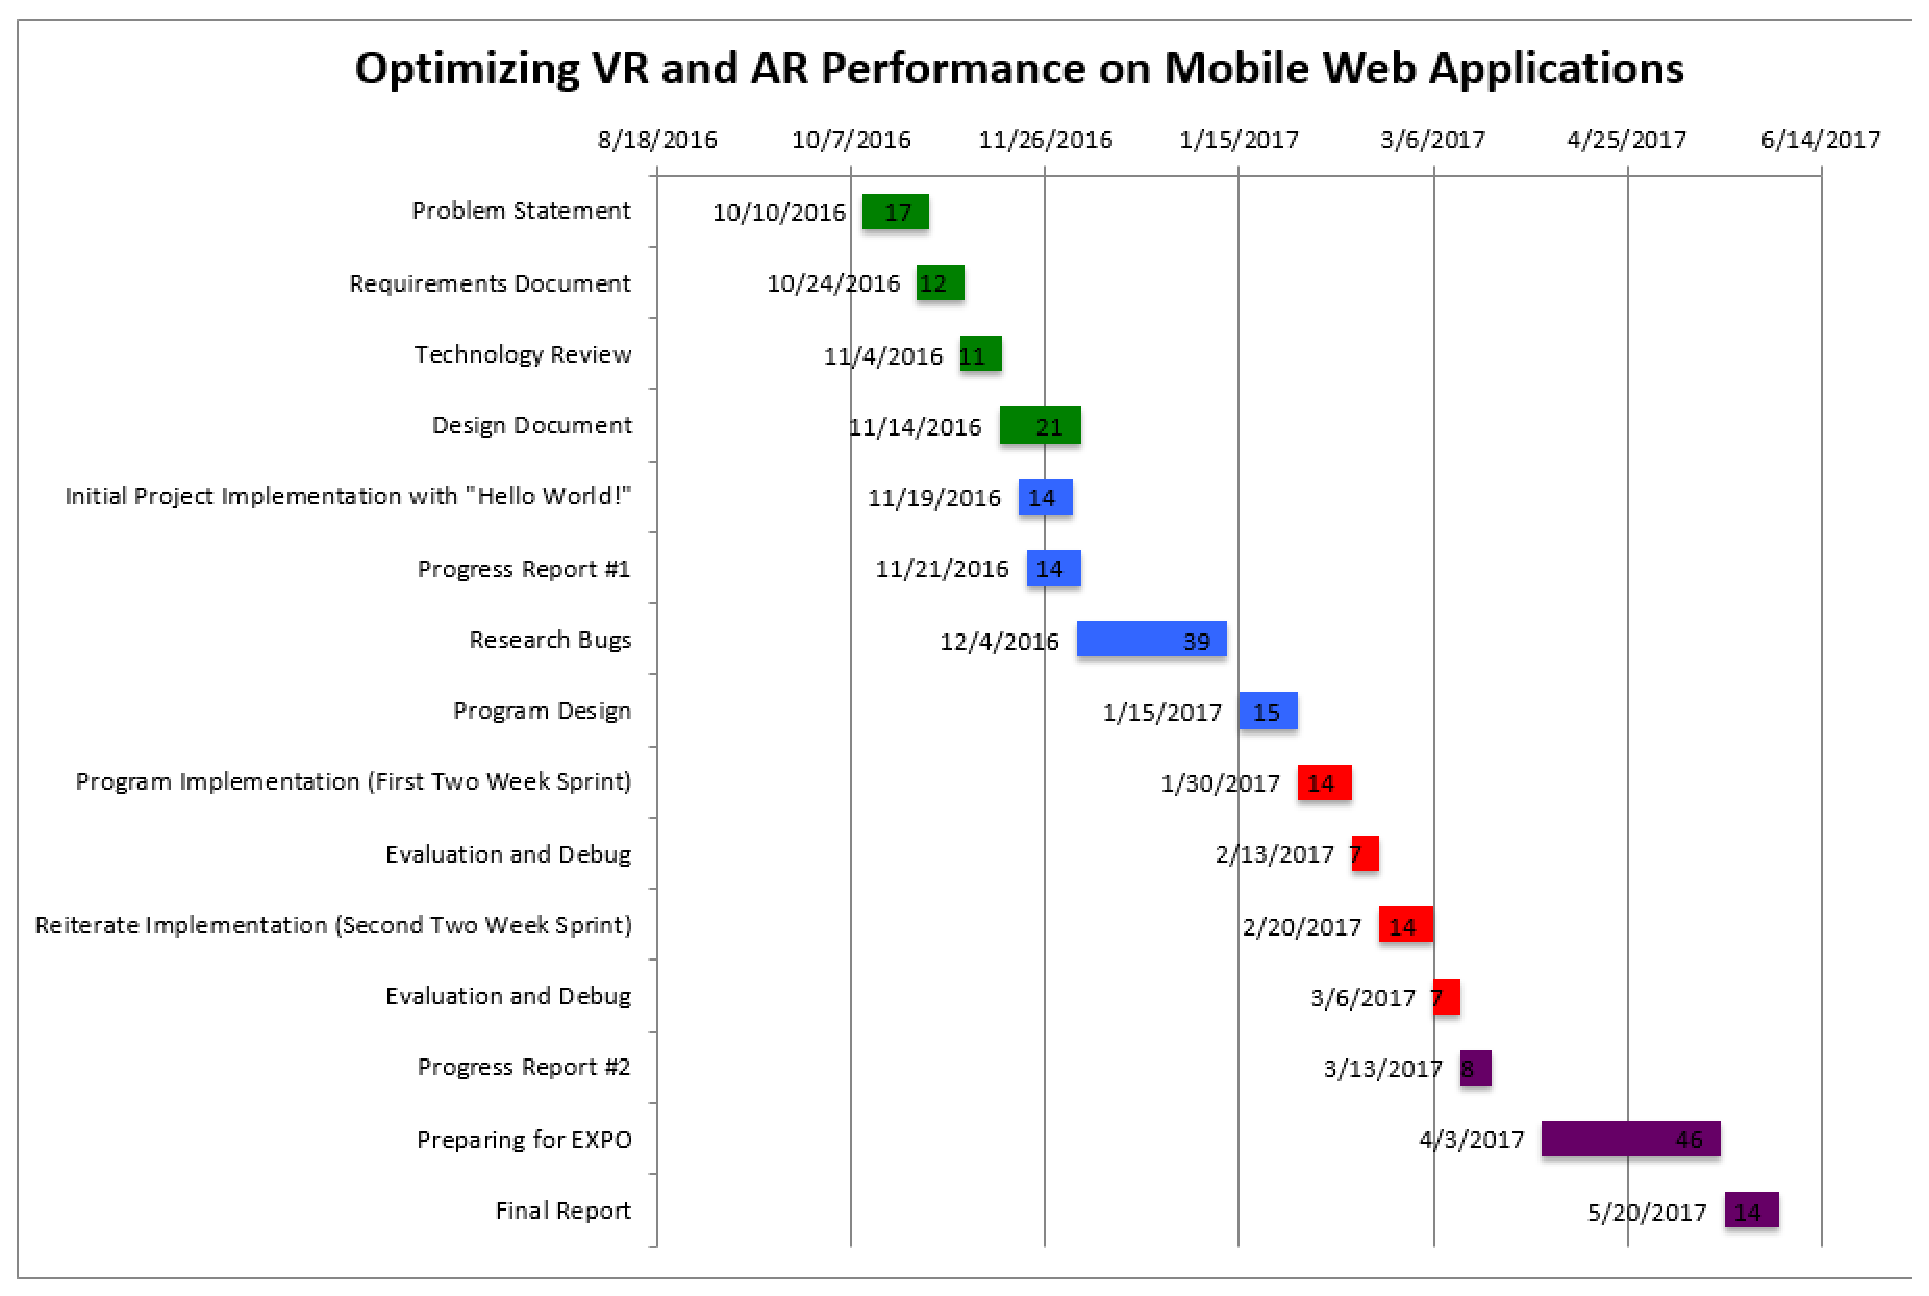
\includegraphics[width=1\textwidth]{OVRAR_Gantt_Chart.eps}
    \end{center}
\end{figure} 
\vfill
\noindent\begin{tabular}{ll}
\makebox[3.5in]{\hrulefill} & \makebox[1.5in]{\hrulefill}\\
Client Signature & Date\\
[4ex]% adds space between the two sets of signatures
\makebox[3.5in]{\hrulefill} & \makebox[1.5in]{\hrulefill}\\
Group Signature & Date\\
[4ex]% adds space between the two sets of signatures
\makebox[3.5in]{\hrulefill} & \makebox[1.5in]{\hrulefill}\\
Group Signature & Date\\
[4ex]% adds space between the two sets of signatures
\makebox[3.5in]{\hrulefill} & \makebox[1.5in]{\hrulefill}\\
Group Signature & Date\\
\end{tabular}
\end{document}